\documentclass[final,5p,times,twocolumn,authoryear]{elsarticle}

\makeatletter
\def\ps@pprintTitle{%
  \let\@oddhead\@empty
  \let\@evenhead\@empty
  \let\@oddfoot\@empty
  \let\@evenfoot\@oddfoot
}
\makeatother

\usepackage{amssymb}
\usepackage{lipsum}
\usepackage{color,soul}
\usepackage{flushend}

\newcommand{\kms}{km\,s$^{-1}$}
\newcommand{\msun}{$M_\odot}

\begin{document}

\begin{frontmatter}

\title{Monte Carlo experiments of network effects in Randomized Controlled Trials}

\author{Márton Trencséni (\texttt{mtrencseni@gmail.com})}

\begin{abstract}
I run Monte Carlo simulations of content production over random Watts-Strogatz graphs to show various effects relevant to modeling and understanding Randomized Controlled Trials on social networks: the network effect, spillover effect, experiment dampening effect, intrinsic dampening effect, clustering effect, degree distribution effect and the experiment size effect. I will also define some simple metrics to measure their strength. When running experiments these potentially unexpected effects must be understood and controlled for in some manner, such as modeling the underlying graph structure to establish a baseline.
 
\end{abstract}

\end{frontmatter}

\section{Introduction}

In academic as well as industry domains \textbf{Randomized Controlled Trials (RCTs)} are the gold standard tool for causal inference. Examples are clinical trials of new drugs and treatments, or improving online services and other online products. One of the core assumptions of traditional RCTs is the \textbf{Independence Assumption (IA)}, that the units of experimentation are independent of each other. In plain words, the assumption is that units don't communicate with each other, they do not affect other units' outcomes based on their own experiences --- whether they are in treatment or control. For many experiments ran on online services however --- social networks such as Facebook or Twitter/X --- the IA does not hold. The simplest toy example considered in this paper is a scenario of a treatment applied to a group of users that is intended to increase their content production. Increased content production of treatment users may boost content production of control users, since they will see their treatment friend's additional posts in their feed, and thus be motivated or inclined to themselves post more. In this paper I consider this toy model, and examine various, potentially unexpected effects that affect (contaminate) an experiment run under such circumstances on a network, where the IA does not hold. To aid the discussion, I will also define some simple metrics to measure the strength of these effects.

\section{Effects considered in this paper}

To discuss and understand these network effects, the paper uses Monte Carlo simulations of RCTs of content production over random Watts-Strogatz graphs. The effects considered and discussed in this paper are:

\begin{itemize}
\setlength\itemsep{0em}
    \item \textbf{Network effect}: each node's neighbours' content production boosts the node's own content production.
    \item \textbf{Degree distribution effect}: the network effect boost is a function of the graph's degree distribution.
    \item \textbf{Spillover effect}: in an experiment that boosts intrinsic content production in a subset of the nodes (the \textit{treatment group}), this boost will spill over to the rest of the nodes.
    \item \textbf{Experiment dampening effect}: due to the spillover effect, we underestimate the lift in the treatment group as compared to control.
    \item \textbf{Intrinsic dampening effect}: the full lift of the treatment group is not realized in the network due to content production in the rest of the network being lower.
    \item \textbf{Clustering effect}: a more tightly clustered treatment group leads to higher lift compared to control.
    \item \textbf{Experiment size effect}: as we add more nodes to the treatment group, absolute content production increases in the treatment group (and the entire network) due to the network effects, but not relative to the control group.
\end{itemize}

\begin{figure}[h]
	\centering 
	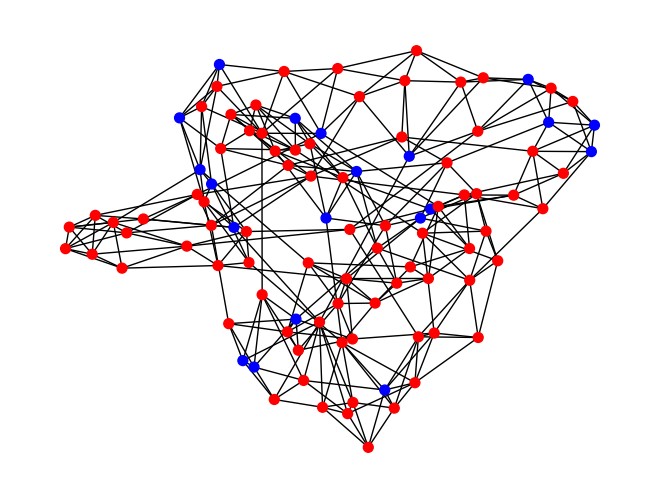
\includegraphics[width=0.4\textwidth]{figure-1.png}	
	\caption{Watts-Strogatz graph with $(n=100, k=6, p=0.1)$, with $N=20$ random treatment nodes colored blue.} 
\end{figure}

\section{Models of content production}

The network is modeled as graph $G = (V, E)$, where $V$ are nodes and $E$ are edges. For simplicity we assume edges are bi-directional, in other words the modeled relationship between nodes (such as \textit{friendship}) is symmetric. Each node $i$ has an associated random variable $R_i$, which describes the node's propensity for content production. Furthermore, we assume the content production random variables $R_i$ follow the same distribution $R$ and are parameterized by a variable $\lambda_i$, such that $R_i = R(\lambda_i)$. Without loss of generality, we will also assume that the random variables have an expectation value, and that $E[R_i] = E[R(\lambda_i)] = \mu_i$. Specifically, we will parameterize the distributions such that $E[R_i] = E[R(\lambda_i)] = \lambda_i$. Note that in some of the Monte Carlo simulations, in cases when we are investigating the mean behaviour, \textit{we will replace the random variable with its mean} --- after verifying this is justified!

We construct a dynamic model of $T$ discrete time steps: let $c_i^t$ be the amount of content produced by node $i$ at time step $t$. At $t=0$ all nodes have 0 content: $c_i^{t=0}=0$. In subsequent time steps, we use the random variables $R(\lambda_i)$ for each node $i$ to model content production, in other words $c_i^t \leftarrow R(\lambda_i^t)$, where $\leftarrow$ denotes drawing a value from the random variable. Note that we will omit indexes and superscripts at times to aid readability. We model the $\lambda_i$ as having two components $\lambda_i = \lambda_{int} + \nu_i$. The first parameter $\lambda_{int}$ models the node's \textit{intrinsic} propensity to produce content, independent of the rest of the graph, and is the same for all nodes on a network. When we model experiments, it is the overall $\lambda$ that will get boosted by $\Delta \lambda$ for treatment nodes, like $\lambda_i = (\lambda_{int} + \nu_i)(1 + \Delta \lambda)$ --- this overall boost simplifies reasoning about the toy models. The second parameter $\nu_i$ models the propensity of the node to produce more content if its neighbours produce more content. We model $\nu_i$ as some function $f$ of the node's neighbours content production in the previous time step: $\nu_i^t = f(c_j^{t-1})$, where $j$ runs for all of $i$'s neighbours. Specifically, we will use $\nu_i^t = \nu_{damp} \sum_{j \in V_i}{c_j^{t-1}}$, where $V_i$ is the set of nodes that are $i$'s neighbours. $\nu_{damp}$ is an important global dampening parameter, whose presence is important to make the overall model stable in the steady-state (see next section).

The above model can be summed up as: at each time step $t$, for each node, we add up content produced by its neighbours in the previous time step, multiply by $\nu_{damp} $, add $\lambda_{int}$, and draw with this parameter from the random variable $R$ to get content production at $t$.

Throughout this paper we will use connected Watts–Strogatz random graphs. A Watts–Strogatz graph is described by 3 parameters $(n, k, p)$. First, a regular ring lattice is constructed, a graph with $n$ nodes each connected to $k < n$ neighbors. Then, "shortcuts" are created by replacing some edges as follows: for each original edge $(u, v)$ in the graph, with probability $p$ replace it with a new edge $(u, w)$, where $w$ is randomly chosen. If the process yield a graph that is not connected, then try again until we get a connected graph. Note that the final randomization process does not change the mean degree in the graph, which remains $k$ at every step.

\section{Mean behaviour, stability and the network effect}

In the model constructed, there are two sources of randomness: (i) randomness introduced when the graph is constructed, and (ii) the random variables used in content production (if one is used). As we will see, to understand the network effects discussed in this paper (ii) is not important, and the random variable may be replaced by its mean.

First, to examine the mean behaviour of the model we run simulations on a Watts-Strogatz graph with $(n=10\,000, k=50, p=0.1)$. We look at three models of content production: (i) a uniform distribution $R(\lambda)=U(0, 2 \lambda)$, (ii) a Poisson distribution $R(\lambda)=Pois(\lambda)$, and (iii) the mean constant case $R(\lambda)=\lambda$. Note that in all three cases, the mean is $E[R(\lambda)]=\lambda$.

Figure 2 shows that content production stabilizes after about $T=10$ steps, and that that in all three cases mean content production across the network is the same, apart from random fluctuations coming from the random variables. Note that in case (i) and (iii) content production is modeled to be continuous, whereas in case of (ii) it's discrete, since the Poisson is a discrete random variable. Figure 3 shows the histogram of content production across nodes in the last time step, for all three models considered.

\begin{figure}[h]
	\centering 
	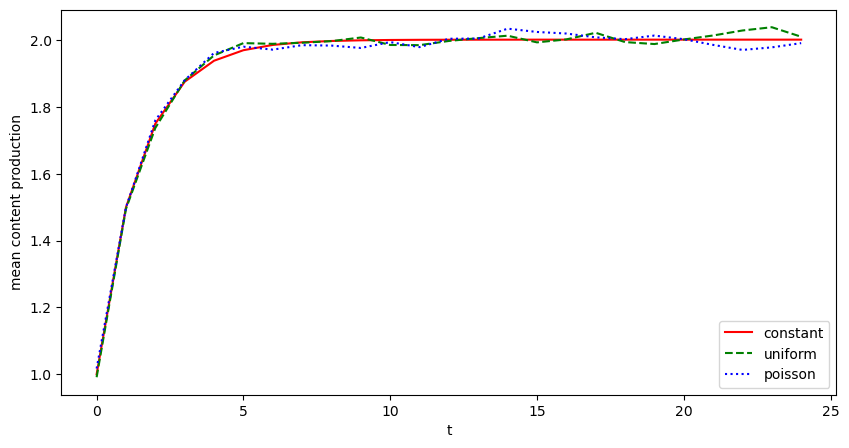
\includegraphics[width=0.4\textwidth]{figure-2.png}	
	\caption{Content production on Watts-Strogatz graph with $(n=10\,000, k=50, p=0.1)$, $\lambda_{int} = 1$ and $\nu_{damp} = 0.01$. Mean content production converges.} 
\end{figure}

\begin{figure}[h]
	\centering 
	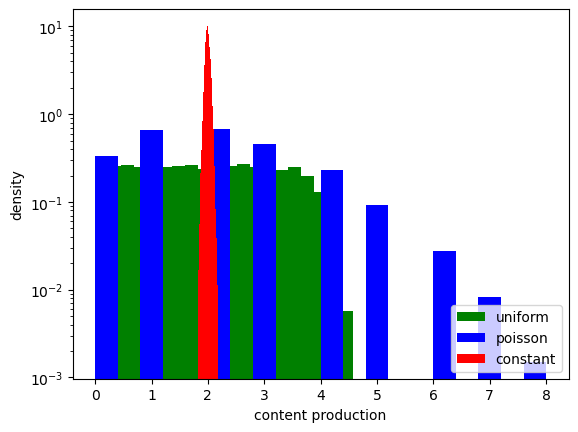
\includegraphics[width=0.4\textwidth]{figure-3.png}	
	\caption{Density histogram of content production during the last step of Monte Carlo simulation for the previous models. The y-axis is logarithmic to ease readability.} 
\end{figure}

In Figure 2, mean content production clearly stabilized. Next, let's re-run the same simulations, but on a Watts-Strogatz graph with $k=200$. The results are shown on Figure 4.

\begin{figure}[h]
	\centering 
	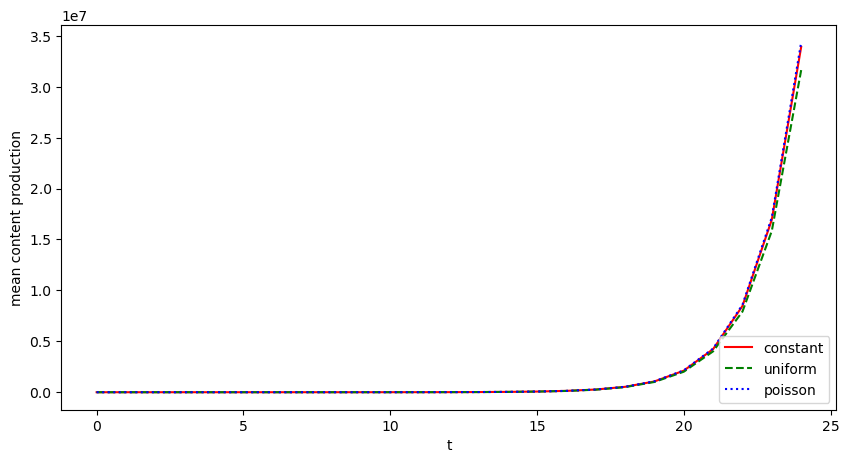
\includegraphics[width=0.4\textwidth]{figure-4.png}	
	\caption{Content production on Watts-Strogatz graph with $(n=10\,000, k=200, p=0.1)$, $\lambda_{int} = 1$ and $\nu_{damp} = 0.01$. Mean content production diverges.} 
\end{figure}

With these parameters content production diverges, it does not reach a steady-state as before. Consider the mean constant case  to see why: assume that the model reaches a steady-state mean content production $c_{base}$. Then, from the way the model is constructed it follows that (using $E[R(\lambda)]=\lambda$):

\begin{equation}
    c_{base} = \lambda_{int} + c_{base} \cdot \bar{V_i} \cdot \nu_{damp}
\end{equation}

where $\bar{V_i}$ is the average number of neighbours per node, which for the Watts-Strogatz graph is $\bar{V_i} = k$ always. Solving for $c_{base}$ we get:

\begin{equation}
    c_{base} = \frac{\lambda_{int}}{ 1 - k \cdot \nu_{damp} }
\end{equation}

For the first model with $\lambda_{int} = 1, k = 50, \nu_{damp} = 0.01$ this yield $c_{base}=2$, which matches the numeric results. Clearly, this equation yields the stability condition:

\begin{equation}
    k \cdot \nu_{damp} < 1
\end{equation}

For the divergent case, the above inequality is not satisfied. It is interesting to see the case where the denominator in Equation (2) is exactly 0, which we can achieve by setting $k=50$. In this case, content production does not explode, but increases linearly indefinitely.

\begin{figure}[h]
	\centering 
	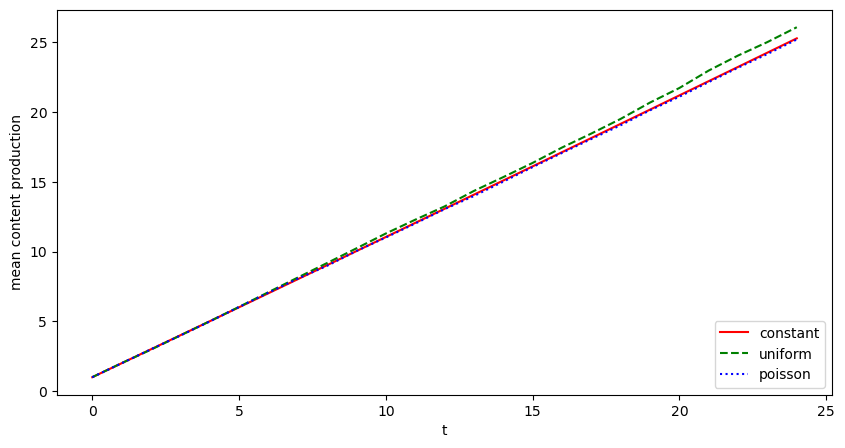
\includegraphics[width=0.4\textwidth]{figure-5.png}	
	\caption{Same as before, with $k=100$.} 
\end{figure}

This simple experiment of Figure 2 shows the \textbf{network effect}: we parameterized intrinsic content production with $\lambda_{int}=1$, which itself, without the boost from neighbours, would have yielded mean content production $c_{base} = \lambda_{int} = 1 $ in this simple model. However, due to the network effect, which here is a function of $k$ and $\nu_{damp}$, the actual mean content production $c_{base}$ is significantly higher, by a factor of $ \frac{ 1 }{ 1 - k \cdot \nu_{damp} } $.

\section{A note on regularizing models}

Real networks can experience exponential growth for a while, but not indefinitely --- some physical resource, such as people, attention or time runs out eventually. In this sense, the models above have unrealistic or un-physical domains because they can diverge. In principle, we can regularize the model in two places:

\begin{itemize}
\setlength\itemsep{0em}
    \item regularize the network effect: assume that each node can only consume a finite amount $\eta_{max}$ of its neighbours' content in a time step
    \item regularize content production: assume that each node can only produce a finite amount $c_{max}$ content
\end{itemize}

In both cases, the assumption is physical in a real network, because only finite time is available per time step to read or write content.

The simplest way to regularize is to cut off with the $max\{\}$ function, so that $\nu_i^t = max\{ \nu_{max}, \nu_{damp} \sum_{j \in V_i}{c_j^{t-1}} \}$ and $c_i^t \leftarrow max\{ c_{max}, R(\lambda_i^t) \}$. A smooth approach is to use a sigmoid function $\sigma(\cdot)$ to achieve smoother cut-off: $\nu_i^t = \nu_{max} \, \sigma \bigl( \nu_{damp} \sum_{j \in V_i}{c_j^{t-1}} \bigr) $ and $c_i^t \leftarrow c_{max} \, \sigma \bigl( R(\lambda_i^t) \bigr) $.

\begin{figure}[h]
	\centering 
	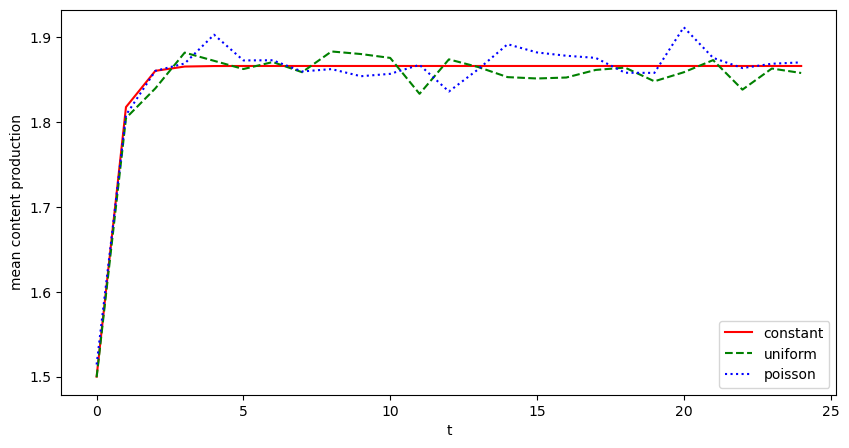
\includegraphics[width=0.4\textwidth]{figure-6.png}	
	\caption{Same as Figure 5, but with regularized network effect using the sigmoid $\sigma(\cdot)$ and $\nu_{max}=1$. Content production is no longer divergent.} 
\end{figure}

Figure 6 shows the same model as Figure 5, but with (just) the network effect regularized. In this case, solving for $c_{base}$ we get:

\begin{equation}
    c_{base} = \lambda_{int} + \nu_{max} \sigma( c_{base} \cdot \bar{V_i} \cdot \nu_{damp} )
\end{equation}

Due to the properties of $\sigma(\cdot)$, there is no closed form solution for $c_{base}$ in this case. In the rest of this paper, we will \textit{not} use regularization, as it makes it harder to reason about the behaviour of the network --- we will work with "raw" models, but always use parameters that yield a stable network.

\section{Degree distribution effect}

In this section we will discuss a small, nuanced adjustment to the above formula for mean content production on a random graph \textit{that is due to the degree distribution of nodes}. In a Watts-Strogatz graph with $p=0$, all nodes have exactly $k$ neighbours; however, at $p>0$, due to the random adjustment of edges, some nodes will end up with lower, and some with higher degree count than $k$. Figure 6 shows the degree distribution of a Watts-Strogatz graph with $k=50$ at different $p$ values. It shows that with increasing $p$, the distribution spreads out around the mean of $k$.

\begin{figure}[h]
	\centering 
	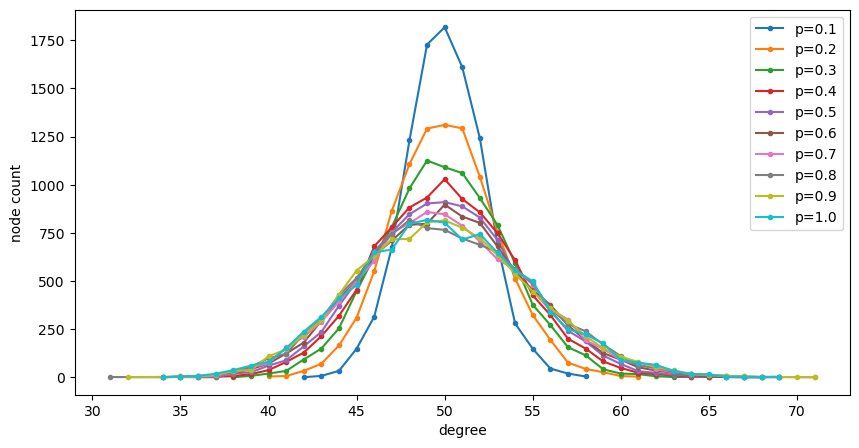
\includegraphics[width=0.4\textwidth]{figure-7.png}	
	\caption{Degree distribution of a Watts-Strogatz with $n=10\,000, k=50$ at different $p$ values.} 
\end{figure}

When examining content production on these random graphs at different $p$ values, an interesting effect shows itself: mean content production increases in a concave way over the base value, which is only realized exactly in the $p=0$ case. Defining

\begin{equation}
    e_{degree\,distribution} = \bar{c} / c_{base} - 1 
\end{equation}

where $\bar{c}$ is the actual content production measured in the network in steady-state and $c_{base}$ is the theoretically calculated value from Equation (2). Figure 8 shows the effect as a function of $p$.

\begin{figure}[h]
	\centering 
	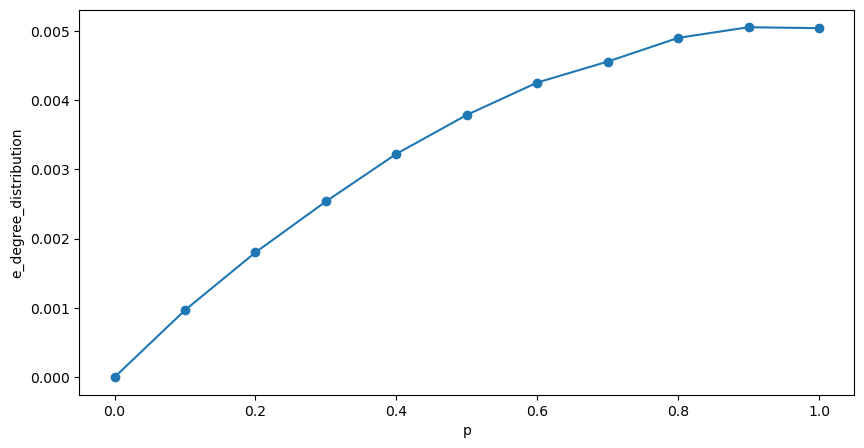
\includegraphics[width=0.4\textwidth]{figure-8.png}	
	\caption{Increased content production due to more spread out degree distribution of a Watts-Strogatz with $n=10\,000, k=50$ at different $p$ values.} 
\end{figure}

The explanation is as follows: the mean degree of nodes remains exactly $k$ in a Watts-Strogatz graph, despite (and during) the final randomization of edges, since the total number of nodes and edges always remains the same. However, as the histogram in Figure 7 shows, some nodes will end up with higher, and some with lower degree, and this is not entirely symmetric: on the lower side, the distribution is more bunched around the mean, whereas on the higher side, the degree distribution moves away further from the mean $k$. As a result, some nodes will have a relatively high neighbour count, get a high network boost, and this is not cancelled out by the nodes having lower degree and experiencing lower network boost, since the distribution is not symmetric. This is illustrated in Figure 9, which shows the mean content production for the same graph as above, but as a function of node degree.

\begin{figure}[h]
	\centering 
	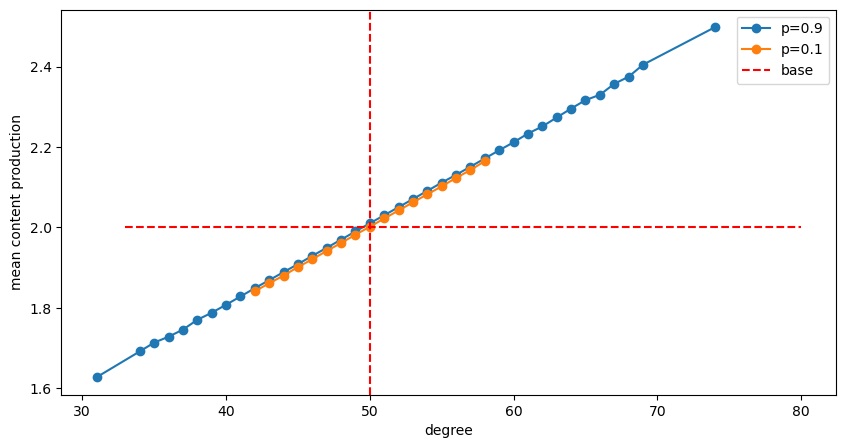
\includegraphics[width=0.4\textwidth]{figure-9.png}	
	\caption{Content production in the previous network, as a function of node degree. The horizontal red dashed line shows the baseline content production we would have without a spread of degree distribution, the vertical red dashed line is the mean degree. Clearly content production is a function of degree, and the spread is wider in the positive direction.} 
\end{figure}

In the rest of the paper we will use the primed notation $c_{base}\prime$ to refer to the "bare" content production on the network, taking into account the above effect (so slightly higher than $c_{base}$). Bare here means no treatment is applied, all nodes are identical. Since there is no known formula for $c_{base}\prime$ to me, it is calculated from a bare Monte Carlo network simulation in the rest of the paper.

\section{Spillover effect}

In this section we will start simulating \textbf{Randomized Controlled Trials (RCTs)} on networks. It's important to point out that RCTs are traditionally run with the \textbf{Independence Assumption (IA)}, that the units of experimentation are independent of each other. In the network models considered here, the IA does not hold --- the resulting behaviour is the topic and \textit{raison d'etre} of this paper itself.

Consider a model on a Watts-Strogatz graph with $(n=500\,000, k=50, p=0.1)$, with identical parameters as before, without regularization. Per Equation (2), such a model has an expected steady-state content production of $c_{base}\prime \approxeq 2$. This base model is modified so that a random 2\% treatment subset of nodes receives a $\Delta \lambda = 0.05$ boost to their overall content production. Figure 10 shows content production separately for \textbf{treatment}, \textbf{neigbhours} of treatment and the \textbf{rest} of nodes (these 3 are distinct sets covering the whole graph).

\begin{figure}[h]
	\centering 
	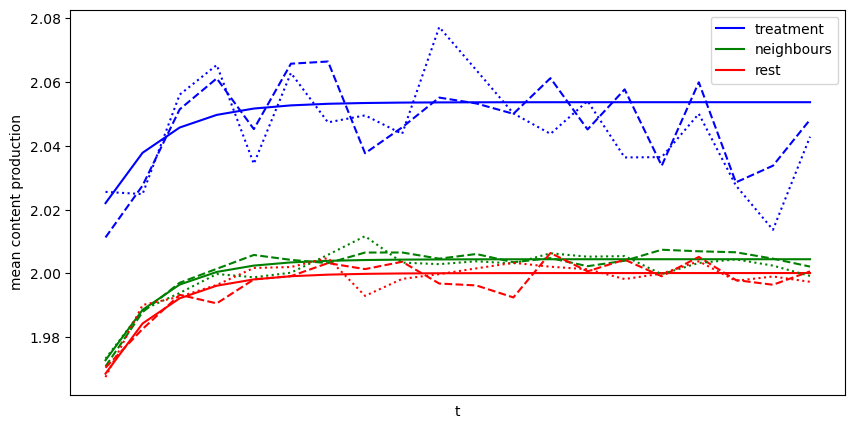
\includegraphics[width=0.4\textwidth]{figure-10.png}	
	\caption{Spillover effect in a Randomized Controlled Trial on a Watts-Strogatz graph with $(n=500\,000, k=50, p=0.1)$ with $N=10\,000$ treatment nodes receiving a $\Delta \lambda = 0.05$ boost to their overall content production, for all three (mean constant, uniform, Poisson) content production models. The line types match the legend on previous figures. The first few time steps where steady-state is approached is not shown.} 
\end{figure}

The following table shows the split of nodes and the average content production $c$ level of the various subsets in the network (\textbf{control} is the union of \textbf{neighbours} and \textbf{rest}):

\begin{center}
\begin{tabular}{ |c|c|c| } 
 \hline
 \textbf{group} & \textbf{cardinality} & $c / c_{base}\prime$ \\ 
 \hline
 treatment   &   $10\,000$   &  1.0258 \\ 
 control     &  $490\,000$   &  1.0005 \\ 
 neighbours  &  $313\,507$   &  1.0012 \\ 
 rest        &  $176\,493$   &  0.9991 \\ 
 \hline
\end{tabular}
\end{center}

What this shows is that the treatment effect \textbf{spills over} into the control group. The spillover is stronger into direct neighbours of treatment, weaker for the rest of nodes. It's also worth noting that treatment, control and neighbours subsets have higher content production than the simulated $c_{base}\prime=2.0019$ base value, which shows that even a small treatment group can "contaminate" the entire network. However, rest (nodes that are not treatment and also not neighbours of treatment) has slightly lower ($c_{rest}/c_{base}\prime < 1$) content production --- how is this possible? The explanation is statistical: the nodes in rest are biased to have less neighbours, in this Monte Carlo simulation their mean degree is $k=49.2$, and this results in this subset's content production being slightly lower due to lower network effects (using the naive formula, $c_{base}(k=49.2)=1.9686$. However, the overall conclusions are unaffected by this observation.

We can measure the strength of the spillover effect by defining:

\begin{equation}
e_{spillover} = c_{control} / c_{base}\prime  - 1
\end{equation}

In other words, $e_{spillover}$ measures the degree of contamination (due to the treatment effect applied to the treatment group). In this scenario we measure $e_{spillover} = 0.0005$.

Clearly, the spillover effect must be a function of $N/n$ and $k$:

\begin{itemize}
\setlength\itemsep{0em}
    \item as $N/n \rightarrow 0, e_{spillover} \rightarrow 0$, because the treatment group becomes insignificant in the overall network
    \item as $k \rightarrow 0, e_{spillover} \rightarrow 0$, because nodes have less neighbours and the model approaches a conventional RCT where the Independence Assumption holds
\end{itemize}

To illustrate the dependence on $N/n$ and $k$, let's look at the same experiment as above, but with $k=10$ and a 1\% treatment group of $N=5\,000$ nodes. In this scenario, where $c_{base}\prime=1.1112$, the mean steady-state of the network is:

\begin{center}
\begin{tabular}{ |c|c|c| } 
 \hline
 \textbf{group} & \textbf{cardinality} & $c / c_{base}\prime$ \\ 
 \hline
 treatment   &  $5\,000$    &  1.0450 \\ 
 control     &  $495\,000$  &  1.0000 \\ 
 neighbours  &  $47\,275$   &  1.0014 \\ 
 rest        &  $447\,725$  &  0.9999 \\ 
 \hline
\end{tabular}
\end{center}

The spillover effect works out to be $e_{spillover}=0.00005$, about 10x weaker than in the previous example.

\begin{figure}[h]
	\centering 
	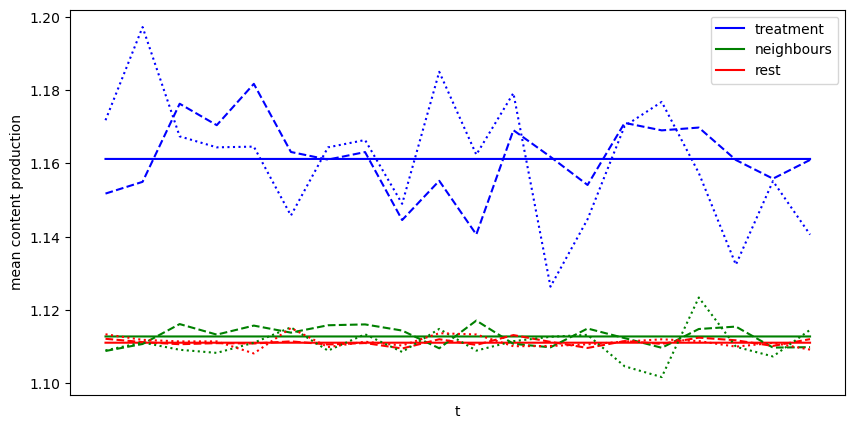
\includegraphics[width=0.4\textwidth]{figure-11.png}	
	\caption{Same as Figure 10, but with $k=10$ and $N=5\,000$.} 
\end{figure}

\section{Experiment dampening effect}

In an RCT, we measure the treatment versus control group lift, and attribute it to be the effect of the applied treatment, with the caveat that one must be careful to separate out signal from noise using statistical hypothesis testing or bayesian inference. In the terminology of this paper, the treatment effect is defined as:

\begin{equation}
e_{treatment} = c_{treatment} / c_{control} - 1
\end{equation}

In the previous two experiments, we measure $e_{treatment} = 0.0253$ and $e_{treatment} = 0.0449$, respectively. Both are lower than the actual treatment effect $\Delta \lambda = 0.05$ we applied synthetically. This is the \textbf{experiment dampening effect}, a result of the spillover effect: because the treatment effect spills over into control and \textit{boosts control as well}, we measure a lower treatment effect. We can define the experiment dampening effect as:

\begin{equation}
e_{dampening} = e_{treatment} / \Delta \lambda
\end{equation}

In the cases above, we get $e_{dampening} = 0.5075$ and $e_{dampening} = 0.8990$, respectively.

\section{Intrinsic dampening effect}

The reason experiments measure treatment against control in traditional RCTs is to factor out seasonal effects. If the experimenter were to compare the treatment group's before-treatment and during-treatment (or after-treatment) metrics, she would not know whether the measured effect is due to the applied treatment, or something else that changed during the experiment. However, in our models, there is no seasonality, so we can examine $c_{treatment}/c_{base}\prime$. Let's define the intrinsic dampening effect:

\begin{equation}
e_{intrinsic} = c_{treatment} / c_{base}\prime - 1
\end{equation}

This measures the dampening in the effect itself due to the connected, non-independent nature of the network. Naively, we may expect that this ratio should be just the applied treatment effect. However, as we will see, this is not the case. Specifically, for the first experiment considered previously, $e_{intrinsic} = 0.0258$, for the second it is $e_{intrinsic} = 0.0450$ (note these are not the same values as for $e_{treatment}$). The full lift is not realized in the treatment group due to content production in the rest of the network being lower, hence, the feedback the treatment nodes receive in their $\nu_i^t = \nu_0 \sum_{j \in V_i}{c_j^{t-1}}$ term is lower. If the entire network were to receive the $\Delta \lambda$ boost, in other words if $N=n$, then the measured $e_{intrinsic} = \Delta \lambda$ would hold, as is evident from Equation (2).

Note that the experiment dampening effect and the intrinsic dampening effect are related, but not the same thing:

\begin{itemize}
\setlength\itemsep{0em}
    \item \textbf{experiment dampening effect}: we underestimate the lift in a treatment versus control measurement due to the treatment effect leaking to the control group in the network at treatment time
    \item \textbf{intrinsic dampening effect}: the full lift of the treatment group is not realized in the network due to content production being lower in the rest of the network (the control group) at treatment time; note that the control group does receive some of the treatment lift, so it's content production also increases, but not to the level of the treatment group
\end{itemize}

\section{Clustering effect}

The clustering effect is a third effect closely related to the previous two: if the treatment nodes are more densely clustered than than the overall graph (or the control group), than the treatment nodes will achieve higher content production, both compared to the control group's $c_{control}$ and the base rate $c_{base}\prime$.

In a randomized test, \textit{on average} the treatment and control's clustering should be the same, but variations may produce higher clustering in treatment; \textit{stratification} controls for this in conventional RCTs. Or, an experiment may have selection bias and thus result is a more clustered treatment group.

To illustrate the effect, let's look at a Monte Carlo run where the treatment nodes are not randomly selected, but significantly more clustered on purpose. To accomplish tighter clustering in a Watts-Strogatz graph is straightforward: instead of randomly selecting nodes, pick a contiguous set of nodes from the original ring (before randomization). At the relatively low $p$ edge randomization values that we're using, this will result in a highly clustered subset.

\begin{figure}[h]
	\centering 
	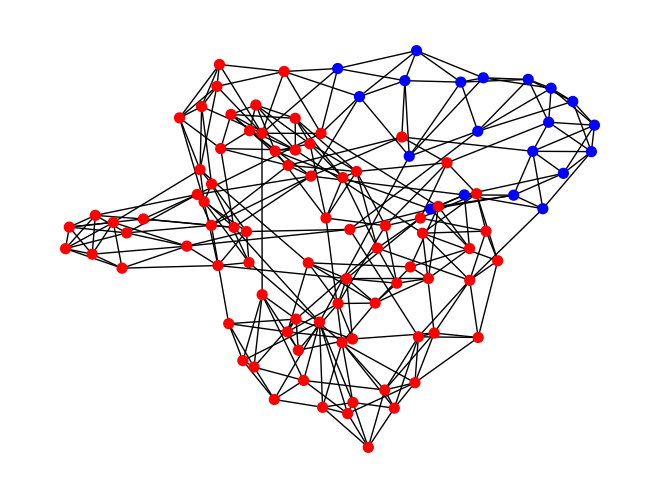
\includegraphics[width=0.4\textwidth]{figure-12.png}	
	\caption{The same Watts-Strogatz graph from Figure 1, but the treatment group is the first 20 nodes from the original ring.} 
\end{figure}

We run an experiment with identical parameters as in Figure 10, except with a much more clustered treatment group: a Watts-Strogatz graph with $(n=500\,000, k=50, p=0.1)$, $\lambda_{int} = 1$ and $\nu_{damp} = 0.01$, with a 2\% treatment group of $N=10\,000$ nodes receiving a $\Delta \lambda = 0.05$ boost to their content production.

\begin{figure}[h]
	\centering 
	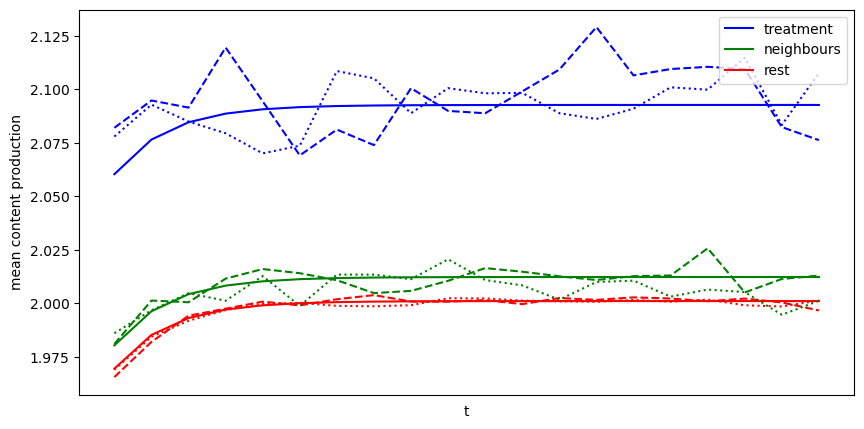
\includegraphics[width=0.4\textwidth]{figure-13.png}	
	\caption{The same Watts-Strogatz graph from Figure 7, but the treatment group is tightly clustered, resulting in significantly higher content production.} 
\end{figure}

However, previously, with a random treatment group the $10\,000$ treatment nodes had $313\,507$ non-treatment neighbours and 37.2\% of treatment node's neighbours were also in treatment, now the $10\,000$ treatment nodes only have $46\,545$ non-treatment neighbours and 90.6\% of treatment node's neighbours are also in treatment. This highly clustered model yields:

\begin{center}
\begin{tabular}{ |c|c|c| } 
 \hline
 \textbf{group} & \textbf{cardinality} & $c / c_{base}\prime$ \\ 
 \hline
 treatment   &  $10\,000$   &  1.0457 \\ 
 control     &  $490\,000$  &  1.0001 \\ 
 neighbours  &  $46\,554$   &  1.0052 \\ 
 rest        &  $443\,446$  &  0.9995 \\ 
 \hline
\end{tabular}
\end{center}

The highly clustered case achieves $e_{dampening} = 0.9136$, so there is barely any dampening, the treatment lift is 91\% of the actual $\Delta \lambda$ lift. The explanation is that 90\% of the treatment group nodes' neighbours are also in treatment, so they get "their own boost back", and there is relatively little dampening. It is also worth noting that $e_{spillover} = 0.0001$, 5x lower than with a truly random treatment group. The explanation is that there are less edges running between treatment and control, so less ways for the spillover to happen.

\section{Experiment size effect}

The last effect we consider is the experiment size effect. The experiment size effect is closely related to the spillover effect, and is simply the observation that with a larger treatment group, there is stronger spillover, which yields stronger feedback, which results in higher content production in the treatment group. Figure 14 shows the variation of $e_{intrinsic}$ with $N/n$ for a Watts-Strogatz graph with $n=10\,000, p=0.1$ and $\Delta \lambda = 0.5$.

\begin{figure}[h]
	\centering 
	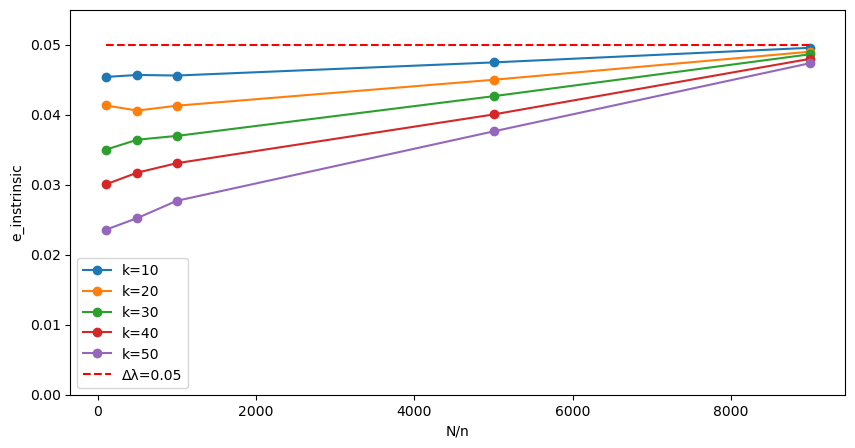
\includegraphics[width=0.4\textwidth]{figure-14.png}	
	\caption{As $N/n$ approaches 1, the intrinsic effect (the ratio of treatment content production to base content production) approaches the experiment effect $\Delta \lambda$. Experiment ran on a Watts-Strogatz graph with $n=10\,000$ and $p=0.1$, at different $k$ values.} 
\end{figure}

However, as pointed out earlier, in an RCT, the experimenter compares treatment content production to control's (and not base). Figure 15 shows $e_{dampening}$ (the ratio of the treatment effect $e_{treatment}$ to the actual $\Delta \lambda$ effect) for the same experiment. Remarkably, the dampening is essentially constant with $N/n$, which means that even with increasing $N$, the experimenter would measure the same treatment effect, because due to spillover, control's content production also goes up.

\begin{figure}[h]
	\centering 
	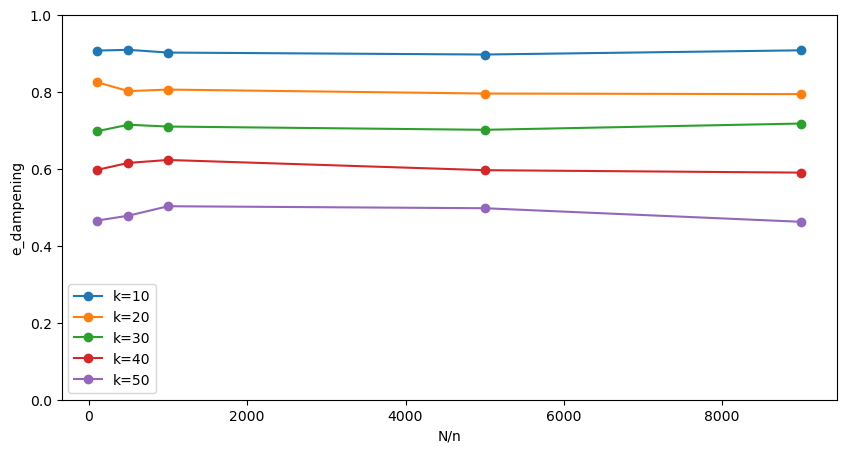
\includegraphics[width=0.4\textwidth]{figure-15.png}	
	\caption{The dampening effect (the ratio of the treatment effect to $\Delta \lambda$) is constant with $N/n$, and is only a function of $k$.} 
\end{figure}

Both plots split as a function of $k$, the mean degree: the lower $k$, the closer we are to the Independence Assumption, the more the measured treatment effect approaches $\Delta \lambda$. Separate experiments (not discussed here) show no dependence on $p$.

\section{Conclusion}

In traditional RCTs where the Independence Assumption holds, the experimenters' main focus is on study design and controlling for statistical fluctuations between the various experiment groups using techniques such as A/A tests, sample size mismatch tests, p-values, Bayesian testing, and so on. This paper showed that when running experiments on social networks or other graphs, where the IA does not hold, various other effects, all a result of the network effect, must be considered and controlled for. As the last section showed, even with high treatment group sizes, due to the treatment effect spilling over to the control group, the experimenter will never measure the true treatment effect when comparing treatment to control. This suggests that in networked conditions measuring or estimating the underlying graph structure and network effects, and then running simulations (similar to the ones in this paper) may be a good method to establish a baseline to compare treatment group behaviour with.

\section{Code}

The paper's accompanying code, including all figures in the paper, is available as a Python notebook on Github. The random seed has been set to a fixed value in the code, so all numerical results are reproducible by re-running the notebook. Use the below link to access the notebook:
\texttt{{\scriptsize https://github.com/mtrencseni/monte-carlo-network-effects-rct-2023 }}

\bibliographystyle{elsarticle-harv} 

\begin{thebibliography}{00}

\bibitem[Kohavi (2020)]{Kohavi2020} Kohavi, Tang, and Xu (2020). \textit{Trustworthy Online Controlled Experiments: A Practical Guide to A/B Testing.} Cambridge University Press.

\bibitem[Watts, Strogatz (1998)]{WattsStrogatz1998} Watts, Strogatz (1998). \textit{Collective dynamics of 'small-world' networks.} Nature. 393 (6684): 440–442.

\bibitem[Barabási (2002)]{Barabasi2002} Albert, Barabási (2002). \textit{Statistical mechanics of complex networks.} Reviews of Modern Physics. 74 (1): 47–97. arXiv:cond-mat/0106096.

\end{thebibliography}

\end{document}

\endinput
